\documentclass{beamer}

\usetheme[sectionpage=simple, subsectionpage=simple,
numbering=fraction, progressbar=none]
{metropolis}

\usepackage[utf8]{inputenc}
\usepackage{graphicx}
\graphicspath{{./img/}}
\usepackage{tikz}

\title{Discrete Random Variables}
\date{\today}
\author{Gonzalo G. Peraza Mues}
% \institute{Universidad Politécnica de Yucatán}

\titlegraphic{
\includegraphics[height=1.5cm]{logo-upy}}

\newcommand{\E}{\operatorname{E}}
\newcommand{\Var}{\operatorname{Var}}

\begin{document}
\maketitle

\begin{frame}{Definition: Random Variable}
  A \alert{random variable} is a function that maps events from a random
  experiments to numerical values.

  \begin{center}
    \textbf{Example}

    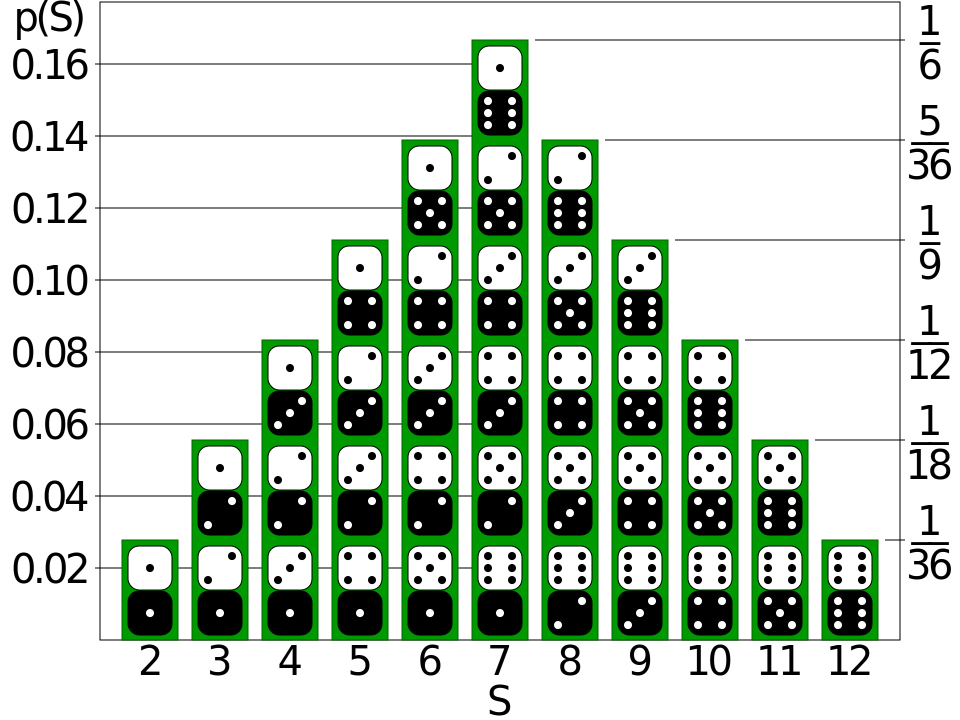
\includegraphics[width=0.6\linewidth]{dice-dist-bar}
  \end{center}
\end{frame}

\begin{frame}{Example: Sexes of 3 children}
  \begin{align*}
    \begin{split}
      S = \{&(b, b, b), (b, b, g), (b, g, b), (b, g, g),\\
      &(g, b, b), (g, b, g), (g, g, b), (g, g, g)\}
    \end{split}
  \end{align*}
  Let $X$ be the number of female children.
  \begin{align*}
    P(X=0) =& \frac{1}{8}\\
    P(X=1) =& \frac{3}{8}\\
    P(X=2) =& \frac{3}{8}\\
    P(X=3) =& \frac{1}{8}\\
  \end{align*}
\end{frame}

\begin{frame}{Discrete Random Variable}
  A random variable is said to be \alert{discrete} if its possible values
  constitute a sequence of \alert{separated points} on the number line.

  $P(X=x_i)$ is the probability that $X=x_i$.

  The collection of these probabilities is called the \alert{probability
    distribution} of $X$
  \begin{align*}
    \sum_{i=1}^n P(X=x_i) = 1
  \end{align*}
\end{frame}

\begin{frame}[t]{Example}
  Suppose that $X$ is a random variable that takes on one of the values 1, 2, or
  3. If
  \begin{align*}
    P(X=1) = 0.4\quad\text{and}\quad P(X=2) = 0.1
  \end{align*}
  what is $P(X=3)$?
\end{frame}

\begin{frame}[t]{Example}
  A saleswoman has scheduled two appointments to sell encyclopedias. She feels
  that her first appointment will lead to a sale with probability 0.3. She also
  feels that the second will lead to a sale with probability 0.6 and that the
  results from the two appointments are independent. What is the probability
  distribution of X, the number of sales made?

  $X$ can take on values 0, 1, 2.
\end{frame}

\begin{frame}{Expected Value}
  The \alert{expected value} of $X$ is a \alert{weighted average} of the
  possible values of $X$:
  \begin{align*}
    \E[X] = \sum_{i=1}^n x_i P(X = x_i)
  \end{align*}
  If $X$ is a random variable associated with some experiment, then the average
  value of $X$ over a large number of replications of the experiment is
  approximately $\E[X]$.
\end{frame}

\begin{frame}[t]{Example}
  Suppose we roll a die that is equally likely to have any of its 6 sides appear
  face up. Find $\E[X]$, where $X$ is the side facing up.
\end{frame}

\begin{frame}[t]{Example}
  Consider a random variable $X$ that takes on either the value 1 or 0 with
  respective probabilities $p$ and $1-p$. That is,
  \begin{align*}
    P(X = 1) = p\quad\text{and}\quad P(X = 0) = 1 - p
  \end{align*}
  Find $\E[X]$.
\end{frame}

\begin{frame}[t]{Example}
  An insurance company sets its annual premium on its life insurance policies
  so that it makes an expected profit of 1 percent of the amount it would have
  to pay out upon death. Find the annual premium on a \$200,000 life insurance
  policy for an individual who will die during the year with probability 0.02.
\end{frame}

\begin{frame}{Properties of expected values}
  \begin{align*}
    \E[cX] =& c\E[X]\\
    \\
    \E[X+c] =& \E[X] + c\\
    \\
    \E[X + Y] =& \E[X] + \E[Y]\\
    \\
    \E\left[ \sum_{i=1}^k X_i\right] =& \sum_{i=1}^k \E[X_i]
  \end{align*}
\end{frame}

\begin{frame}[t]{Example}
  A married couple works for the same employer. The wife’s Christmas bonus is a
  random variable whose expected value is \$1500.
  \begin{enumerate}
  \item If the husband's bonus is set to equal 80 percent of his wife’s, find
    the expected value of the husband’s bonus.
  \item If the husband’s bonus is set to equal \$1000 more than his wife’s, find its
    expected value.
  \end{enumerate}
\end{frame}

\begin{frame}[t,shrink=10]{Example}
  The following table lists the number of civilian full-time law enforcement
  employees in eight cities in 1990.

  \begin{tabular*}{1.0\linewidth}{l c}
    City & Civilian law enforcement employees\\
    \hline
    Minneapolis, MN & 105\\
    Newark, N J & 155\\
    Omaha, NE & 149\\
    Portland, OR & 195\\
    San Antonio, TX & 290\\
    San Jose, CA & 357\\
    Tucson, AZ & 246\\
    Tulsa, OK & 178\\
  \end{tabular*}

  Suppose that two of the cities are to be randomly chosen and all the civilian
  law enforcement employees of these cities are to be interviewed. Find the
  expected number of people who will be interviewed.
\end{frame}

\begin{frame}[t]{Example}
  A building contractor has sent in bids for three jobs. If the contractor
  obtains these jobs, they will yield respective profits of 20, 25, and 40 (in
  units of \$1000).  On the other hand, for each job the contractor does not
  win, he will incur a loss (due to time and money already spent in making the
  bid) of 2. If the probabilities that the contractor will get these jobs are,
  respectively, 0.3, 0.6, and 0.2, what is the expected total profit?
\end{frame}

\begin{frame}{Variance and standard deviation of random variables}
  If $X$ is a random variable with expected value $\mu$, then the variance of
  $X$, denoted by $\Var(X)$, is defined by
  \begin{align*}
    \Var(X) = \E[{(X - \mu)}^2] = \E[X^2] - \mu^2
  \end{align*}
  The standard deviation of $X$, denoted by $SD(X)$, is
  \begin{align*}
    SD(X) = \sqrt{\Var(X)}
  \end{align*}
\end{frame}

\begin{frame}[t]{Example}
  Find $\Var(X)$ when the random variable $X$ is such that
  \begin{align*}
    X=
    \begin{cases}
      1 & \text{with probability }p\\
      0 & \text{with probability }1-p
    \end{cases}
  \end{align*}
\end{frame}

\begin{frame}[t]{Example}
  The return from a certain investment (in units of \$1000) is a random variable
  $X$ with probability distribution
  \begin{align*}
    P(X=-1) = 0.7 \quad
    P(X=4) = 0.2 \quad
    P(X=8) = 0.1
  \end{align*}
  Find $\Var(X)$, the variance of the return.
\end{frame}

\begin{frame}{Properties of variances}
  \begin{align*}
    \Var(cX) =& c^2\Var(X)\\
    \\
    \Var(X+c) =& \Var(X)
  \end{align*}
\end{frame}

\begin{frame}{Independent random variables}
  Random variables $X$ and $Y$ are \alert{independent} if knowing the value of one of them
  does not change the probabilities of the other.

  If $X$ and $Y$ are independent random variables, then
  \begin{align*}
    \Var(X + Y) = \Var(X) + \Var(Y )
  \end{align*}
  More generally
  \begin{align*}
    \Var\left( \sum_{i=1}^k X_i \right) = \sum_{i=1}^k \Var (X_i)
  \end{align*}
\end{frame}

\begin{frame}[t]{Example}
  Determine the variance of the sum obtained when a pair of fair dice is rolled.
\end{frame}

\begin{frame}[t]{Example}
  The annual gross earnings of a certain rock singer are a random variable with
  an expected value of \$400,000 and a standard deviation of \$80,000. The
  singer’s manager receives 15 percent of this amount. Determine the expected
  value and standard deviation of the amount received by the manager.
\end{frame}

\begin{frame}{The urn problem}
  Pick a ball, return the ball. Repeat n times.

  What is the probability of picking $X$ red balls?

  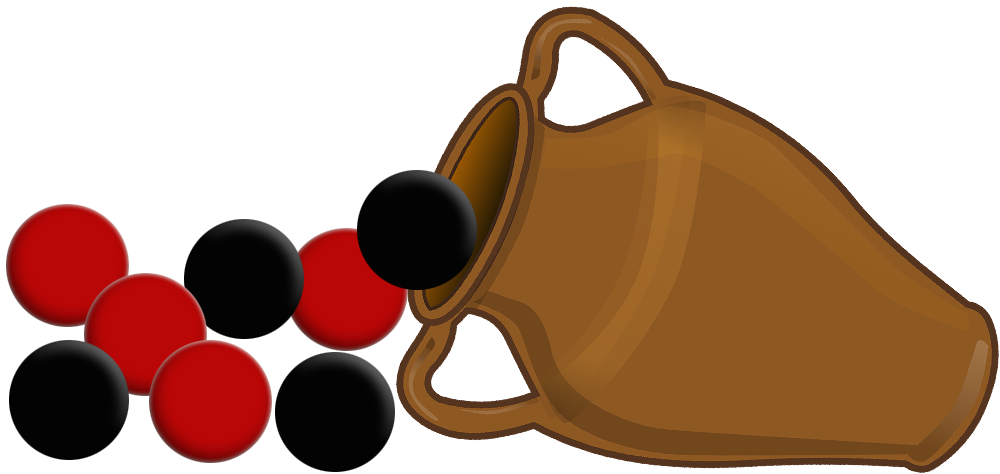
\includegraphics[width=\linewidth]{urn2_small}
\end{frame}

\begin{frame}{Binomial Random Variables}
  A \alert{binomial random variable} with parameters \alert{n} and \alert{p}
  represents the number of \alert{successes} in \alert{n} independent
  \alert{trials}, when each trial is a success with probability $p$.  If $X$is
  such a random variable, then for $i = 0, \ldots , n$, the probability mass
  function is
  \begin{align*}
    P(X=i) = \frac{n!}{i!(n-i)!}p^i {(1-p)}^{n-i}
  \end{align*}
  and the cumulative distribution function is
  \begin{align*}
    P(X \leq j) = \sum_{i=0}^j \binom n i p^i {(1-p)}^{n-i}
  \end{align*}
\end{frame}

\begin{frame}{Probability mass function}
  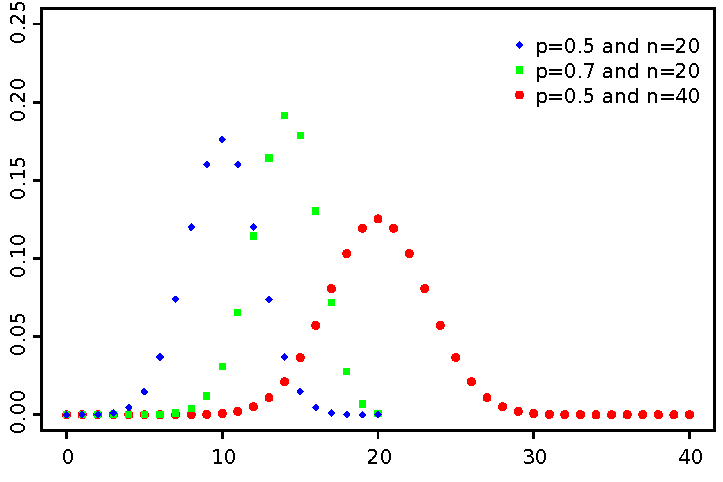
\includegraphics[width=\linewidth]{Binomial_distribution_pmf}
\end{frame}

\begin{frame}{Cumulative distribution function}
  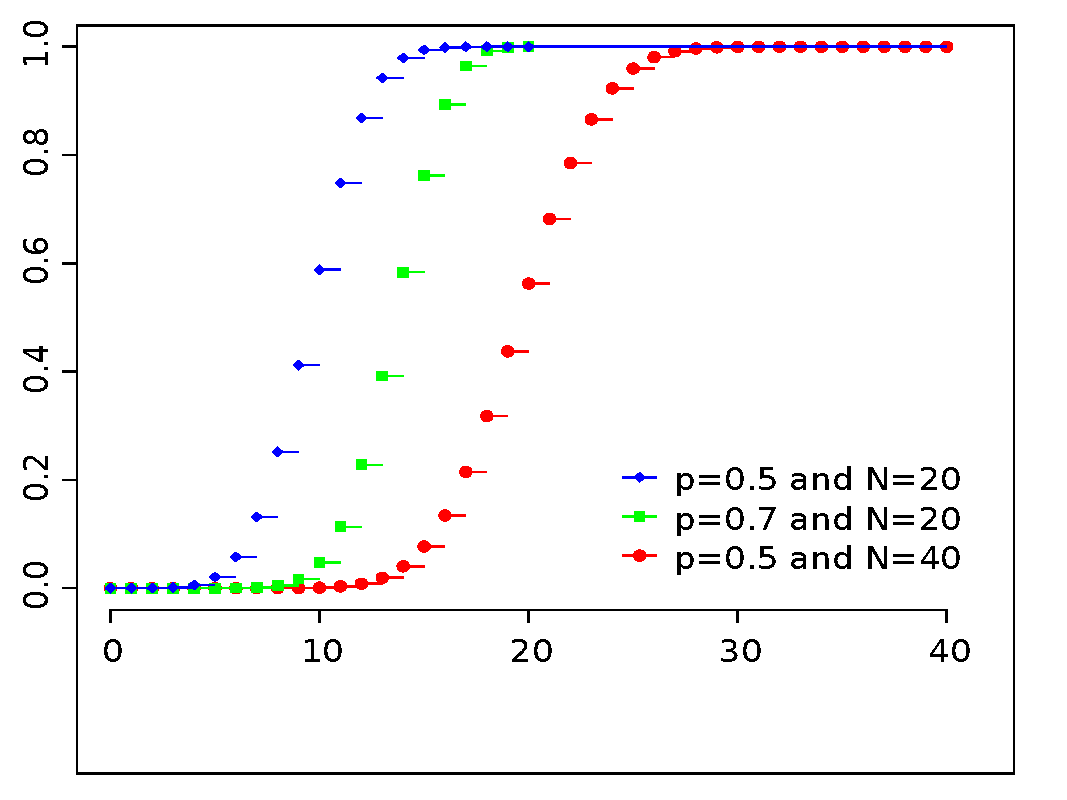
\includegraphics[width=\linewidth]{Binomial_distribution_cdf}
\end{frame}

\begin{frame}[t]{Example}
  Three fair coins are flipped. If the outcomes are independent, determine the
  probability that there are a total of $i$ heads, for $i = 0, 1, 2, 3$.
\end{frame}

\begin{frame}[t,shrink=20]{Example}
  Suppose that a particular trait (such as eye color or handedness) is
  determined by a single pair of genes, and suppose that $d$ represents a
  dominant gene and $r$ a recessive gene. A person with the pair of genes
  $(d, d)$ is said to be pure dominant, one with the pair $(r, r)$ is said to be
  pure recessive, and one with the pair $(d, r)$ is said to be hybrid. The pure
  dominant and the hybrid are alike in appearance. When two individuals mate,
  the resulting offspring receives one gene from each parent, and this gene is
  equally likely to be either of the parent’s two genes.
  \begin{enumerate}
  \item What is the probability that the offspring of two hybrid parents has the
    opposite (recessive) appearance?
  \item Suppose two hybrid parents have 4 offsprings. What is the probability 1
    of the 4 offspring has the recessive appearance?
  \end{enumerate}
\end{frame}

\begin{frame}[t]{Example}
  \begin{enumerate}
  \item Determine $P(X \leq 12)$ when $X$ is a binomial random variable with
    parameters 20 and 0.4.
  \item Determine $P(Y \leq 10)$ when $Y$ is a binomial random variable with
    parameters 16 and 0.5.
  \end{enumerate}
  Use the R function \texttt{pbinom}
\end{frame}

\begin{frame}{Expected Value and Variance of a Binomial Random Variable}
  If $X$ is binomial with parameters $n$ and $p$, then

  \begin{align*}
    \E[X] =& np\\
    \\
    \Var(X) =& np(1 - p)
  \end{align*}

\end{frame}

\begin{frame}[t]{Example}
  Suppose that each screw produced is independently defective with probability
  0.01. Find the expected value and variance of the number of defective screws
  in a shipment of size 1000.
\end{frame}

\begin{frame}{The urn problem, again}
  Pick a ball, keep the ball. Repeat n times.

  What is the probability of picking $X$ red balls?

  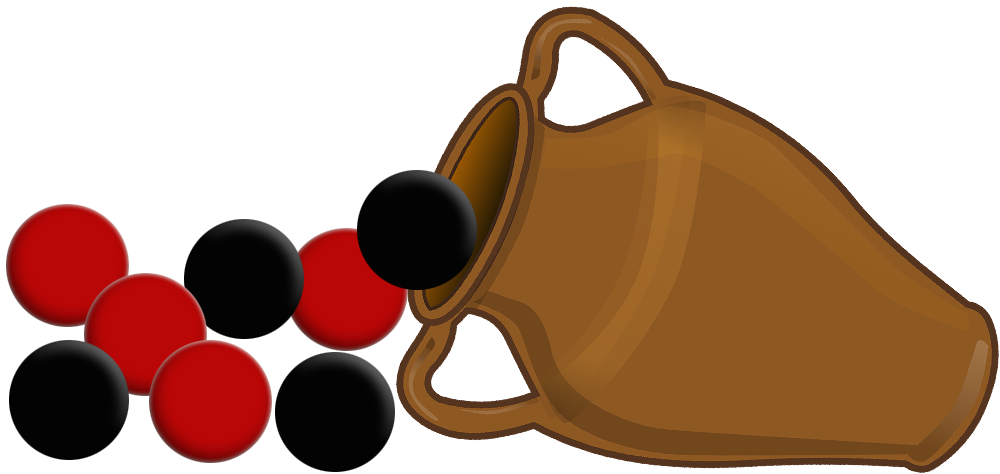
\includegraphics[width=\linewidth]{urn2_small}
\end{frame}

\begin{frame}{Hypergeometric Distribution}
  The hypergeometric distribution describes the probability of \alert{X}
  successes in \alert{n} draws, without replacement, from a finite population of
  size \alert{N} that contains exactly \alert{K} successes. The probability mass
  function is
  \begin{align*}
    P(X=i) = \frac{\binom K i \binom {N-K} {n-i} }{\binom {N} {n}}
  \end{align*}

  When N is large in relation to n, and p=K/N, a hypergeometric random variable
  with parameters n, N, K approximately has a binomial distribution with
  parameters n and p.
\end{frame}

\begin{frame}{Expected Value and Variance for a Hypergeometric distribution}
  \begin{align*}
    \E[X] =& np\\
    \\
    \Var(X) =& \frac{N - n}{N - 1} np(1 - p)
  \end{align*}
\end{frame}

\begin{frame}[t]{Example}
  If 6 people are randomly selected from a group consisting of 12 men and 8
  women, then the number of women chosen is a hypergeometric random variable
  with parameters $n = 6$, $N = 20$, $p = 8/20 = 0.4$. Similarly, the number of
  men chosen is a hypergeometric random variable with parameters $n = 6$, $N = 20$,
  $p = 0.6$. What is the mean and variance of both groups?
\end{frame}

\begin{frame}{Poisson Random Variables}
  A random variable $X$ is called a \alert{Poisson} random variable with
  parameter $\lambda$ if
  \begin{align*}
    P(X=i) = \frac{e^{-\lambda}\lambda^i}{i!},\quad i=0,1,\ldots
  \end{align*}

  Binomial random variables with large values of n and small values of p can be
  approximated by a Poisson random variable with $\lambda=np$.

  If $X$ is a Poisson random variable with parameter $\lambda > 0$, then
  \begin{align*}
    \E[X] =& \lambda\\
    \Var(x) =& \lambda
  \end{align*}

\end{frame}

\begin{frame}[t]{Example}
  Suppose that items produced by a certain machine are independently defective
  with probability 0.1. What is the probability that a sample of 10 items will
  contain at most 1 defective item? What is the Poisson approximation for this
  probability?
\end{frame}

\begin{frame}[t]{Example}
  Suppose the average number of accidents occurring weekly on a particular
  highway is equal to 1.2. Approximate the probability that there is at least one
  accident this week.
\end{frame}

\begin{frame}{The Poisson Distribution}
  It expresses the probability of a given number of events occurring in a fixed
  interval of time and/or space if these events occur with a known average rate
  ($\lambda$) and \alert{independently} of the time since the last event.

  Examples:
  \begin{itemize}
  \item The number of meteors greater than 1 meter diameter that strike earth in
    a year.
  \item The number of patients arriving in an emergency room between 11 and 12 pm.
  \end{itemize}
\end{frame}

\begin{frame}{Probability mass function}
  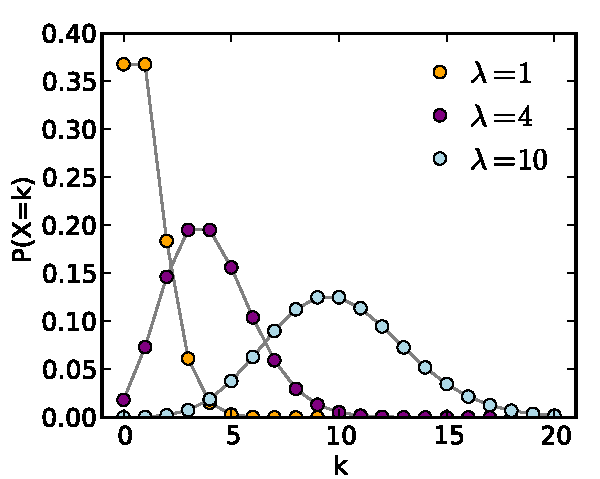
\includegraphics[width=0.9\linewidth]{Poisson_pmf}
\end{frame}

\begin{frame}{Cumulative distribution function}
  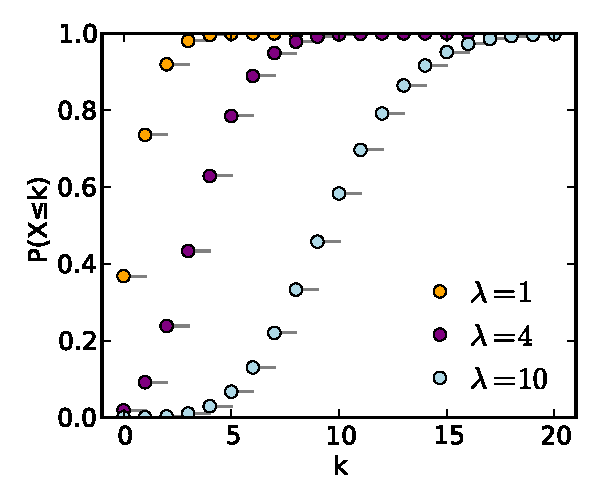
\includegraphics[width=0.9\linewidth]{Poisson_cdf}
\end{frame}

\begin{frame}[t]{Example}
  On a particular river, overflow floods occur once every 100 years on
  average. Calculate the probability of k = 0, 1, 2, 3, 4, 5, or 6 overflow
  floods in a 100-year interval, assuming the Poisson model is appropriate.
\end{frame}

\begin{frame}[t]{Example}
  Ugarte and colleagues report that the average number of goals in a World Cup
  soccer match is approximately 2.5 and the Poisson model is appropriate.
\end{frame}

\begin{frame}[t]{Derivation}
  The Poisson distribution is the limit of the Binomial distribution as a
  function of $\lambda = np$ when $n\rightarrow \infty$. Hint: $e^x =
  \lim_{n\rightarrow \infty} (1+x/n)^n$.
\end{frame}
\end{document}

%%% Local Variables:
%%% mode: latex
%%% TeX-master: t
%%% End:
